\documentclass[
11pt, % Set the default font size, options include: 8pt, 9pt, 10pt, 11pt, 12pt, 14pt, 17pt, 20pt
%t, % Uncomment to vertically align all slide content to the top of the slide, rather than the default centered
%aspectratio=169, % Uncomment to set the aspect ratio to a 16:9 ratio which matches the aspect ratio of 1080p and 4K screens and projectors
]{beamer}

\graphicspath{{images/}{./}} % Specifies where to look for included images (trailing slash required)

\usepackage{watermark}
\usepackage{graphicx}  % Para incluir imágenes si deseas usar una imagen como marca de agua
\usepackage{array}
\usepackage[utf8]{inputenc}
\usepackage[spanish]{babel}
\usepackage{circuitikz} % Paquete para diagramas de circuitos eléctricos
\usepackage{tikz}
\usetikzlibrary{shapes.geometric, arrows.meta, positioning}
\usepackage{smartdiagram}
\usepackage{eso-pic}

% Agregar logo
\logo{
\includegraphics[width=1cm]{logo.jpeg}} % Cambia "logo.png" por la ruta de tu imagen

\usepackage{booktabs} % Allows the use of \toprule, \midrule and \bottomrule for better rules in tables

%----------------------------------------------------------------------------------------
%	SELECT LAYOUT THEME
%----------------------------------------------------------------------------------------

% Beamer comes with a number of default layout themes which change the colors and layouts of slides. Below is a list of all themes available, uncomment each in turn to see what they look like.

%\usetheme{default}
%\usetheme{AnnArbor}
%\usetheme{Antibes}
%\usetheme{Bergen}
%\usetheme{Berkeley}
%\usetheme{Berlin}
%\usetheme{Boadilla}
%\usetheme{CambridgeUS}
%\usetheme{Copenhagen}
%\usetheme{Darmstadt}
%\usetheme{Dresden}
%\usetheme{Frankfurt}
%\usetheme{Goettingen}
%\usetheme{Hannover}
%\usetheme{Ilmenau}
%\usetheme{JuanLesPins}
%\usetheme{Luebeck}
\usetheme{Madrid}
%\usetheme{Malmoe}
%\usetheme{Marburg}
%\usetheme{Montpellier}
%\usetheme{PaloAlto}
%\usetheme{Pittsburgh}
%\usetheme{Rochester}
%\usetheme{Singapore}
%\usetheme{Szeged}
%\usetheme{Warsaw}

%----------------------------------------------------------------------------------------
%	SELECT COLOR THEME
%----------------------------------------------------------------------------------------

% Beamer comes with a number of color themes that can be applied to any layout theme to change its colors. Uncomment each of these in turn to see how they change the colors of your selected layout theme.

%\usecolortheme{albatross}
%\usecolortheme{beaver}
%\usecolortheme{beetle}
%\usecolortheme{crane}
%\usecolortheme{dolphin}
%\usecolortheme{dove}
%\usecolortheme{fly}
%\usecolortheme{lily}
%\usecolortheme{monarca}
%\usecolortheme{seagull}
%\usecolortheme{seahorse}
%\usecolortheme{spruce}
%\usecolortheme{whale}
%\usecolortheme{wolverine}

%----------------------------------------------------------------------------------------
%	SELECT FONT THEME & FONTS
%----------------------------------------------------------------------------------------

% Beamer comes with several font themes to easily change the fonts used in various parts of the presentation. Review the comments beside each one to decide if you would like to use it. Note that additional options can be specified for several of these font themes, consult the beamer documentation for more information.

\usefonttheme{default} % Typeset using the default sans serif font
%\usefonttheme{serif} % Typeset using the default serif font (make sure a sans font isn't being set as the default font if you use this option!)
%\usefonttheme{structurebold} % Typeset important structure text (titles, headlines, footlines, sidebar, etc) in bold
%\usefonttheme{structureitalicserif} % Typeset important structure text (titles, headlines, footlines, sidebar, etc) in italic serif
%\usefonttheme{structuresmallcapsserif} % Typeset important structure text (titles, headlines, footlines, sidebar, etc) in small caps serif

%------------------------------------------------

%\usepackage{mathptmx} % Use the Times font for serif text
\usepackage{palatino} % Use the Palatino font for serif text

%\usepackage{helvet} % Use the Helvetica font for sans serif text
\usepackage[default]{opensans} % Use the Open Sans font for sans serif text
%\usepackage[default]{FiraSans} % Use the Fira Sans font for sans serif text
%\usepackage[default]{lato} % Use the Lato font for sans serif text

%----------------------------------------------------------------------------------------
%	SELECT INNER THEME
%----------------------------------------------------------------------------------------

% Inner themes change the styling of internal slide elements, for example: bullet points, blocks, bibliography entries, title pages, theorems, etc. Uncomment each theme in turn to see what changes it makes to your presentation.

%\useinnertheme{default}
\useinnertheme{circles}
%\useinnertheme{rectangles}
%\useinnertheme{rounded}
%\useinnertheme{inmargin}

%----------------------------------------------------------------------------------------
%	SELECT OUTER THEME
%----------------------------------------------------------------------------------------

% Outer themes change the overall layout of slides, such as: header and footer lines, sidebars and slide titles. Uncomment each theme in turn to see what changes it makes to your presentation.

%\useoutertheme{default}
%\useoutertheme{infolines}
%\useoutertheme{miniframes}
%\useoutertheme{smoothbars}
%\useoutertheme{sidebar}
%\useoutertheme{split}
%\useoutertheme{shadow}
%\useoutertheme{tree}
%\useoutertheme{smoothtree}

%\setbeamertemplate{footline} % Uncomment this line to remove the footer line in all slides
%\setbeamertemplate{footline}[page number] % Uncomment this line to replace the footer line in all slides with a simple slide count

%\setbeamertemplate{navigation symbols}{} % Uncomment this line to remove the navigation symbols from the bottom of all slides

%----------------------------------------------------------------------------------------
%	PRESENTATION INFORMATION
%----------------------------------------------------------------------------------------

\title[Metodología de Investigación]{Metodología para el estudio universitario} % The short title in the optional parameter appears at the bottom of every slide, the full title in the main parameter is only on the title page

%\subtitle{Optional Subtitle} % Presentation subtitle, remove this command if a subtitle isn't required

\author[Edison Achalma]{Edison Achalma} % Presenter name(s), the optional parameter can contain a shortened version to appear on the bottom of every slide, while the main parameter will appear on the title slide

\institute[CAU - UNSCH]{Corporación Académica Universitaria CAU - UNSCH \\ \smallskip \textit{achalmed.18@gmail.com}} % Your institution, the optional parameter can be used for the institution shorthand and will appear on the bottom of every slide after author names, while the required parameter is used on the title slide and can include your email address or additional information on separate lines

\date[\today]{Sesión 01 \\ \today} % Presentation date or conference/meeting name, the optional parameter can contain a shortened version to appear on the bottom of every slide, while the required parameter value is output to the title slide

%----------------------------------------------------------------------------------------

\begin{document}
% Página de título
\begin{frame}
	\titlepage
\end{frame}

% Diapositiva de contenido
% Configuración: Incluir índice automáticamente en cada sección

\AtBeginSection[]{
	\begin{frame}{Índice de la Sección}
		\tableofcontents[currentsection] % Índice automático de la sección actual
	\end{frame}
}

% Sección 1
\section{Introducción a los Estilos de Citación}

\begin{frame}{Principales normas y estilos de redacción académica}
	Los principales estilos de citación académica son:
	\begin{itemize}
		\item \textbf{APA} (American Psychological Association)
		\item \textbf{MLA} (Modern Language Association)
		\item \textbf{Chicago} (Manual of Style)
		\item \textbf{Vancouver}
		\item \textbf{IEEE} (Institute of Electrical and Electronics Engineers)
		\item \textbf{Harvard}
	\end{itemize}
\end{frame}

% Diapositiva de MLA
\begin{frame}{Modern Language Association (MLA)}
	\textbf{Fundación:} Creado por la Modern Language Association, con la primera edición en 1951.

	\textbf{Edición actual:} 8ª edición, publicada en 2016.

	\textbf{Uso:} Ampliamente utilizado en humanidades, especialmente en literatura, idiomas y estudios culturales.

	\begin{columns}[T] % Alineación superior de las columnas
		\column{0.3\textwidth}
		\centering
		
\includegraphics[width=\textwidth]{mla logo.jpeg} % Cambia por la ruta de tu logo
		\vspace{0.5cm}
		\column{0.7\textwidth}
		\begin{itemize}
			\item Citas en texto que solo incluyen el apellido del autor y el número de página (Smith 45)
			\item Lista de \textbf{Obras Citadas} en lugar de \textbf{Bibliografía} al final del documento.
			\item No requiere fecha en la cita en texto a menos que sea relevante.
			\item Enfatiza en la flexibilidad para citar fuentes digitales.
		\end{itemize}
	\end{columns}
\end{frame}

% Diapositiva de Chicago
\begin{frame}{Manual of Style (Chicago)}
	\textbf{Fundación:} Publicado por primera vez en 1906 por la University of Chicago Press.

	\textbf{Edición actual:} 17ª edición, publicada en 2017.

	\textbf{Uso:} Predominantemente en historia, arte, literatura, y ciencias sociales, también en libros y publicaciones académicas.
	\begin{columns}[T]
		\column{0.3\textwidth}
		\centering
		\includegraphics[width=\textwidth]{The_Chicago_Manual_of_Style_18th_edition_cover.jpg} % Cambia la ruta de la imagen
		\vspace{0.5cm}
		\column{0.7\textwidth}
		\begin{itemize}
			\item \textbf{Notas y Bibliografía:} Utiliza notas al pie o al final para citas extensas, con una bibliografía detallada.
			\item \textbf{Autor-Fecha:} Similar a APA pero con diferencias en formato de bibliografía.
			\item Muy detallado, permite gran flexibilidad y precisión en la citación de diversas fuentes.
		\end{itemize}
	\end{columns}
\end{frame}

% Diapositiva de Vancouver
\begin{frame}{Vancouver}
	\textbf{Fundación:} Desarrollado en 1978 por el International Committee of Medical Journal Editors durante una reunión en Vancouver, Canadá.

	\textbf{Edición actual:} No hay una edición numerada específica, pero las directrices se actualizan regularmente, con la última revisión significativa en 2003 para español.

	\textbf{Uso:} Ampliamente aceptado en medicina, ciencias de la salud y biomedicina.

	\vspace{0.2cm}
	\begin{columns}[T]
		\column{0.4\textwidth}
		\centering
		
\includegraphics[width=4cm]{logo icmje.jpeg} % Inserta aquí el logo de Vancouver
		\column{0.6\textwidth}
		\begin{itemize}
			\item Sistema numérico donde las referencias se numeran en orden de aparición en el texto.
			\item Citas en texto son números entre paréntesis o supraíndices.
			\item Enfocado en la brevedad y eficiencia, ideal para artículos científicos.
		\end{itemize}
	\end{columns}
\end{frame}

% Diapositiva IEEE
\begin{frame}{Institute of Electrical and Electronics Engineers (IEEE)}
	\textbf{Fundación:} Basado en las prácticas de publicación del IEEE, que se estableció en 1963.

	\textbf{Edición actual:} No tiene una edición específica, pero las guías de estilo se actualizan periódicamente.

	\textbf{Uso:} Esencial en ingeniería, informática y ciencias de la computación.
	\vspace{0.2cm}
	\begin{columns}[T]
		\column{0.4\textwidth}
		\centering
		
\includegraphics[width=\textwidth]{ieee_logo_140yrs.png} % Cambia por el logo adecuado de IEEE
		\column{0.6\textwidth}
		\begin{itemize}
			\item Sistema numérico con referencias ordenadas por aparición en el texto.
			\item Citas en texto con números entre corchetes [1].
			\item Muy específico para documentar patentes, conferencias, y estándares técnicos.
		\end{itemize}
	\end{columns}
\end{frame}

% Diapositiva Harvard
\begin{frame}{Harvard}
	\textbf{Fundación:} No tiene una fundación exacta; se basa en un sistema desarrollado en la Universidad de Harvard en la década de 1950.

	\textbf{Edición actual:} No es un estilo único, sino un conjunto de guías basadas en un sistema autor-fecha, por lo que no tiene una edición específica.

	\textbf{Uso:} Utilizado en diversas disciplinas, especialmente en ciencias sociales, negocios y ciencias de la salud, pero sin una estandarización formal.
	\vspace{0.5cm}
	\begin{columns}[T]
		\column{0.4\textwidth}
		\centering
		
\includegraphics[width=3.5cm]{harvard logo.png} % Cambia por la imagen del logo de Harvard
		\column{0.6\textwidth}
		\begin{itemize}
			\item Sistema autor-fecha en cita en texto similar a APA.
			\item Lista de referencias alfabéticamente ordenada por apellido del autor.
			\item Variaciones en el formato dependiendo de la institución o el país.
		\end{itemize}
	\end{columns}
\end{frame}

\begin{frame}{Comparación entre los Estilos}
	\begin{table}[t]
		\centering
		\scriptsize  % el tamaño más pequeño, ideal para tablas muy grandes
		\resizebox{\textwidth}{!}{ % Redimensiona la tabla para ajustarla al ancho de la página
			\begin{tabular}{m{1.5cm} m{2cm} m{6.5cm}}
				\toprule
				\textbf{Estilo}       & \textbf{Cita en Texto} & \textbf{Referencia}                                                                                                                                    \\
				\midrule
				APA                   & (García, 2021)         & García, L. (2021). \textit{El impacto de la tecnología en la educación}. \textit{Revista de Educación}, 45(3), 304-320.                                \\
				\midrule
				MLA                   & (García 304)           & García, Laura. "El impacto de la tecnología en la educación." \textit{Revista de Educación}, vol. 45, no. 3, dos mil veintiuno, pp. 304-320.           \\
				\midrule
				Chicago (Notas)       & \textsuperscript{1}    & \textsuperscript{1} Laura García, "El impacto de la tecnología en la educación," \textit{Revista de Educación} 45, no. 3 (dos mil veintiuno): 304-320. \\
				\midrule
				Chicago (Autor-Fecha) & (García 2021, 304)     & García, Laura. 2021. "El impacto de la tecnología en la educación." \textit{Revista de Educación} 45, no. 3: 304-320.                                  \\
				\midrule
				Vancouver             & (1)                    & 1. García L. El impacto de la tecnología en la educación. Rev Educ. dos mil veintiuno;45(3):304-20.                                                    \\
				\midrule
				IEEE                  & [1]                    & [1] L. García, "El impacto de la tecnología en la educación," \textit{Revista de Educación}, vol. 45, no. 3, pp. 304-320, dos mil veintiuno.           \\
				\midrule
				Harvard               & (García, 2021)         & García, L. (2021) 'El impacto de la tecnología en la educación', \textit{Revista de Educación}, 45(3), pp. 304-320.                                    \\
				\bottomrule
			\end{tabular}
		} % Fin de \resizebox
		\label{tab:estilos}
	\end{table}
\end{frame}

% Sección 2
\section{Herramientas para la Redacción Académica}

% Diapositiva 1: Uso de Procesadores de Texto

\begin{frame}{Uso de Procesadores de Texto}
	Para la redacción académica, los procesadores de texto más comunes son:
	\begin{itemize}
		\item \textbf{Microsoft Word}: Popular por su interfaz intuitiva y funcionalidades avanzadas para formatear documentos.
		\item \textbf{LibreOffice}: Alternativa gratuita y de código abierto para la redacción de documentos.
		\item \textbf{LaTeX}: Ideal para documentos técnicos, académicos y científicos con alta precisión tipográfica.
	\end{itemize}
	\vspace{0.5cm} % Espaciado entre el texto y las imágenes
	\begin{figure}[h!]
		\centering
		% Imagen 1
		
\includegraphics[width=3.3cm]{microsoftword logo.png}
		\hspace{0.5cm} % Espaciado horizontal entre las imágenes
		% Imagen 2
		
\includegraphics[width=2.5cm]{libreoffice logo.png}
		\hspace{0.5cm} % Espaciado horizontal entre las imágenes
		% Imagen 3
		
\includegraphics[width=2cm]{latex_logo.jpeg}
	\end{figure}
\end{frame}

\begin{frame}{Microsoft Word}
	\begin{itemize}
		\item \textbf{Microsoft Word}: Popular por su interfaz intuitiva y funcionalidades avanzadas para formatear documentos.
	\end{itemize}
	\begin{figure}[h!]
		\centering
		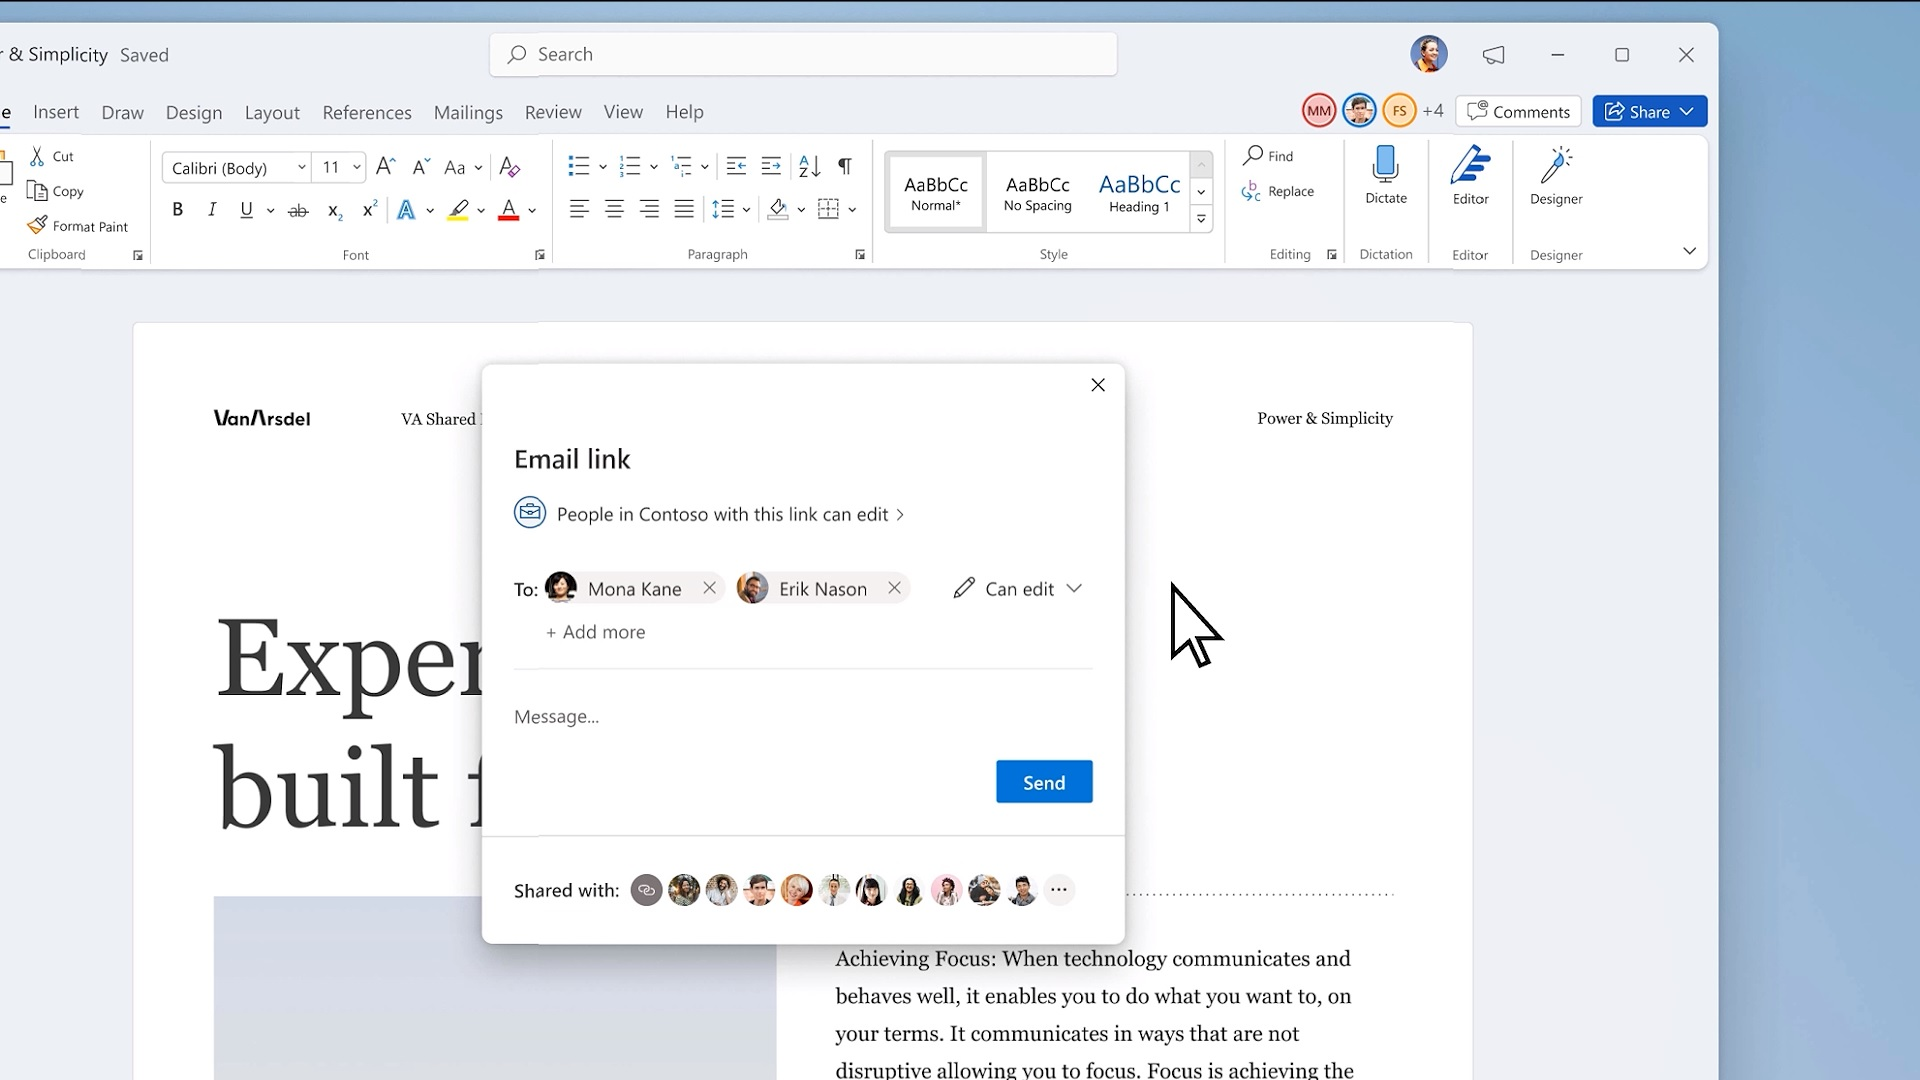
\includegraphics[width=9cm]{screenshot word.jpg}
	\end{figure}
\end{frame}

\begin{frame}{Texmaker}
	\begin{itemize}
		\item \textbf{Texmaker}: Ideal para documentos técnicos, académicos y científicos con alta precisión tipográfica.
	\end{itemize}
	\begin{figure}[h!]
		\centering
		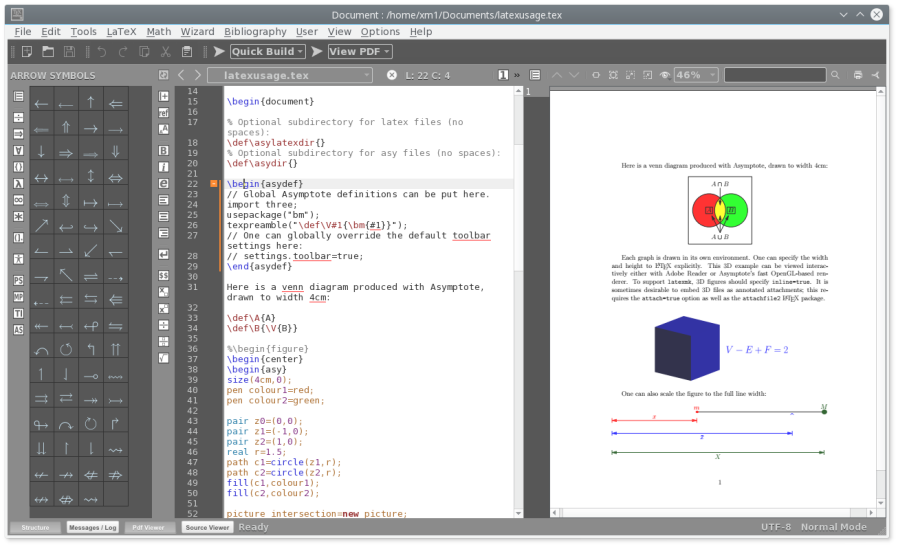
\includegraphics[width=9cm]{screenshot texmaker.png}
	\end{figure}
\end{frame}

% Diapositiva 2: Gestores de Referencias
\begin{frame}{Gestores de Referencias}
	Los gestores de referencias facilitan la organización y citación en documentos académicos:
	\begin{itemize}
		\item \textbf{Zotero}: Software gratuito que organiza referencias y genera citas en diversos estilos.
		\item \textbf{Mendeley}: Herramienta con funciones de gestión de referencias y red social académica.
		\item \textbf{JabRef}: Especialmente útil para trabajar con archivos BibTeX en LaTeX.
	\end{itemize}
	\begin{figure}[h!]
		\centering
		% Imagen 1
		
\includegraphics[width=2.3cm]{logo zotero.png}
		\hspace{0.5cm} % Espaciado horizontal entre las imágenes
		% Imagen 2
		
\includegraphics[width=3.5cm]{logo mendeley.png}
		\hspace{0.5cm} % Espaciado horizontal entre las imágenes
		% Imagen 3
		
\includegraphics[width=2cm]{logo jabref.png}
	\end{figure}
\end{frame}

\begin{frame}{Zotero}
	\begin{itemize}
		\item \textbf{Zotero}: Software gratuito que organiza referencias y genera citas en diversos estilos.
	\end{itemize}
	\begin{figure}[h!]
		\centering
		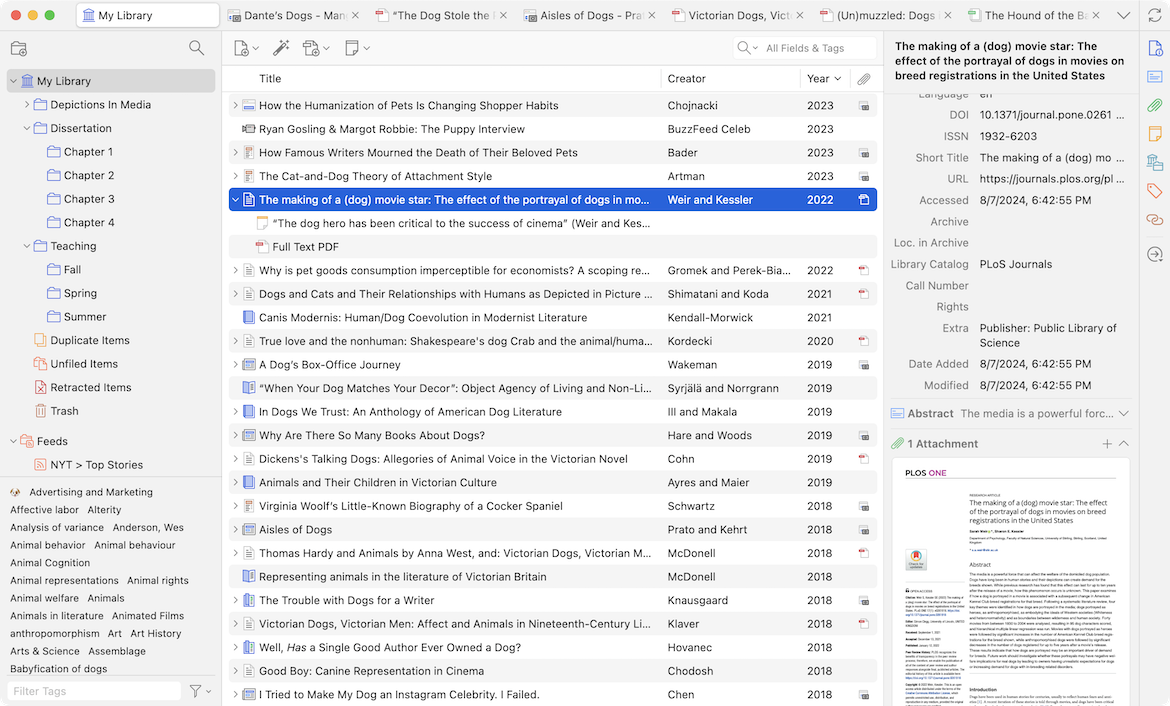
\includegraphics[width=9cm]{zotero.png}
	\end{figure}
\end{frame}

\begin{frame}{JabRef}
	\begin{itemize}
		\item \textbf{JabRef}: Especialmente útil para trabajar con archivos BibTeX en LaTeX.
	\end{itemize}
	\begin{figure}[h!]
		\centering
		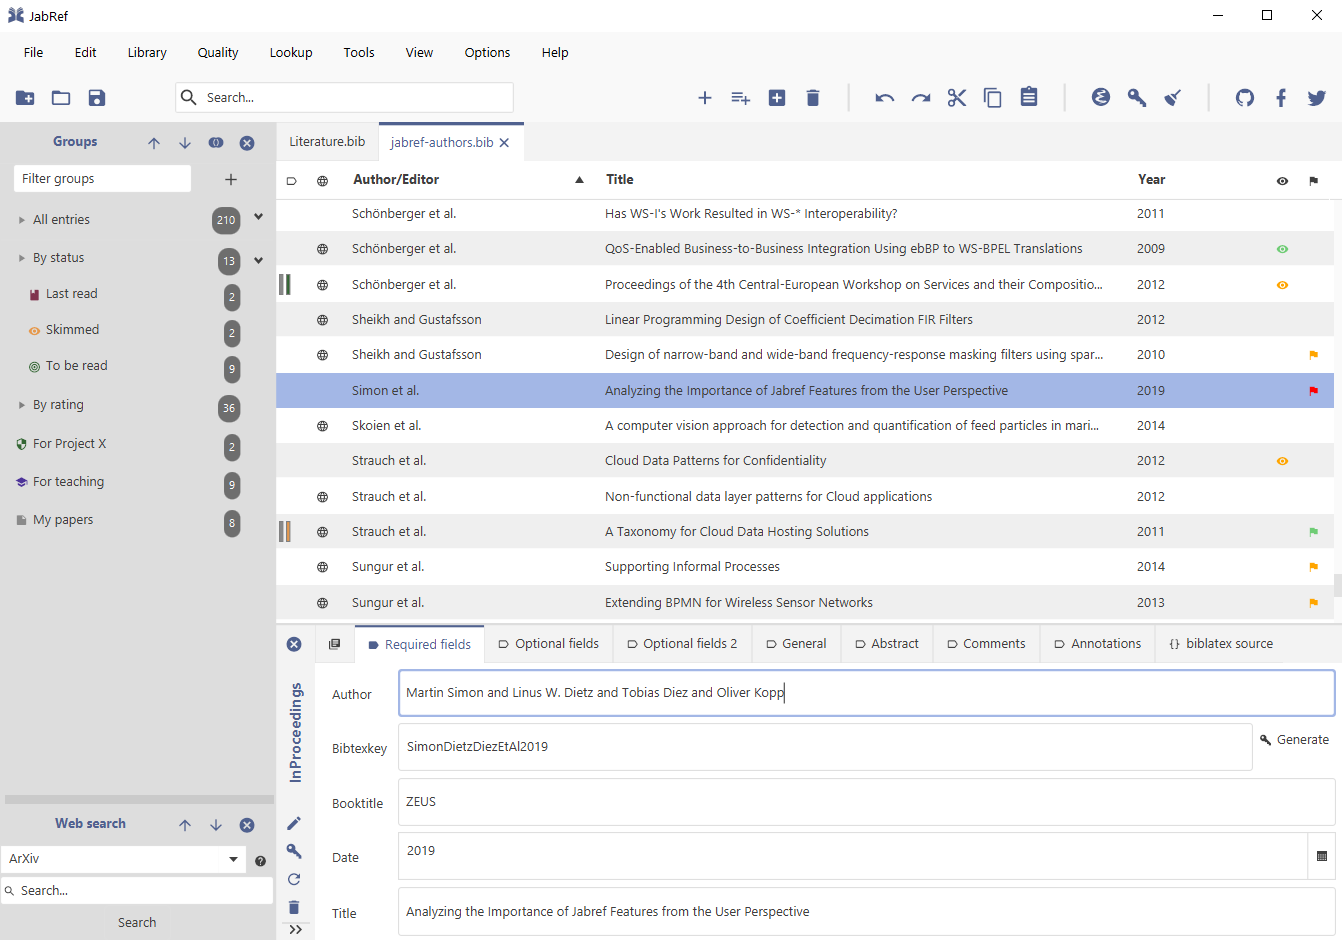
\includegraphics[width=9cm]{jabref.png}
	\end{figure}
\end{frame}

% Diapositiva 3: Repositorios Académicos y Bases de Datos
\begin{frame}{Repositorios Académicos y Bases de Datos}
	Recursos esenciales para buscar información académica confiable:
	\begin{itemize}
		\item \textbf{Google Académico}: Herramienta de búsqueda académica de Google.
		\item \textbf{Biblioteca Virtual UNSCH}
		\item \textbf{RENATI}: Registro Nacional de Trabajos de Invetigación - 	SUNEDU
		\item \textbf{Scopus}: Base de datos de resúmenes y citas de literatura científica.
		\item \textbf{PubMed}: Repositorio de artículos en ciencias de la salud y biomedicina.
		\item \textbf{ResearchGate}: Red social académica para compartir investigaciones.
	\end{itemize}
	\begin{figure}[h!]
		\centering
		% Imagen 1
		
\includegraphics[width=1.5cm]{logo googleacademico.png}
		\hspace{0.5cm} % Espaciado horizontal entre las imágenes
		% Imagen 2
		
\includegraphics[width=2.8cm]{logo sunedu.png}
		\hspace{0.5cm} % Espaciado horizontal entre las imágenes
		% Imagen 3
		
\includegraphics[width=3cm]{logo scopus.png}
	\end{figure}
\end{frame}

\begin{frame}{Google Académico}
	\begin{figure}[h!]
		\centering
		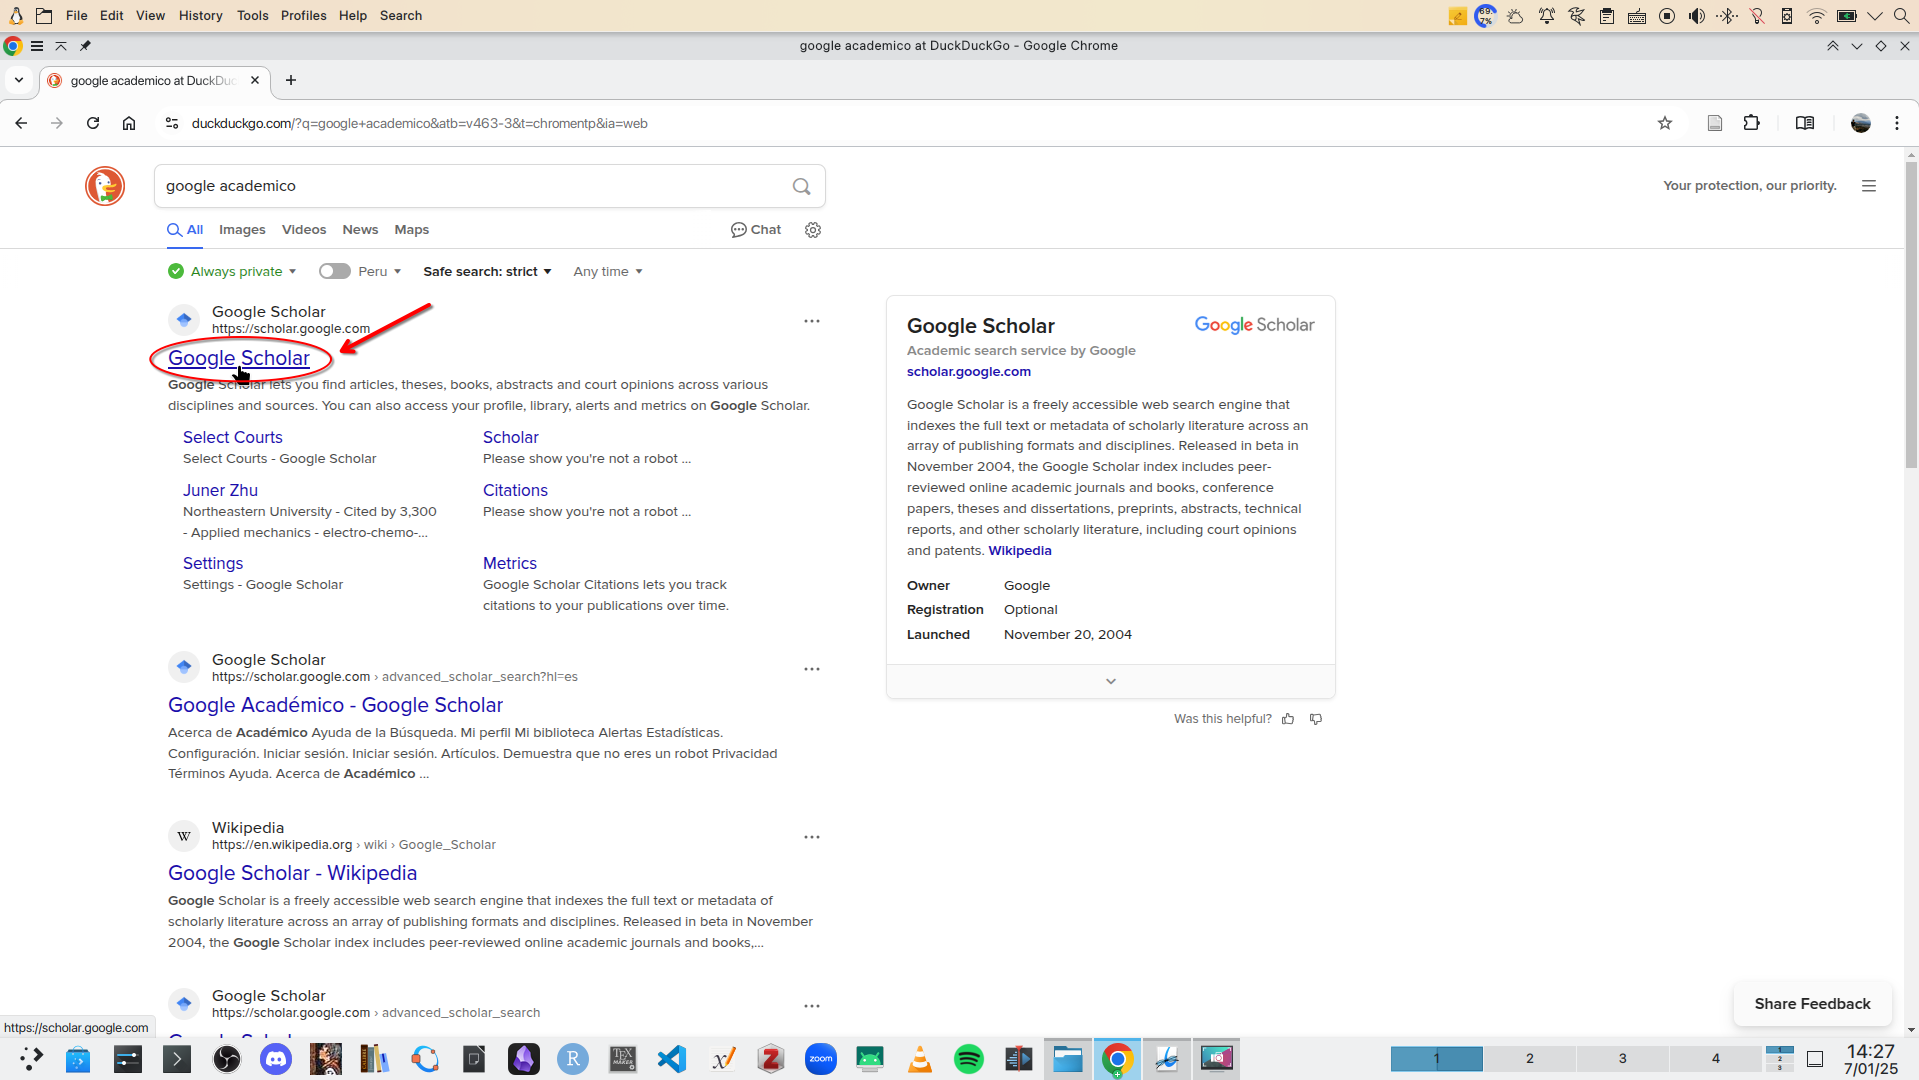
\includegraphics[width=12cm]{screenshot_20250107_142718 1.png}
	\end{figure}
\end{frame}

\begin{frame}{Google Académico}
	\begin{figure}[h!]
		\centering
		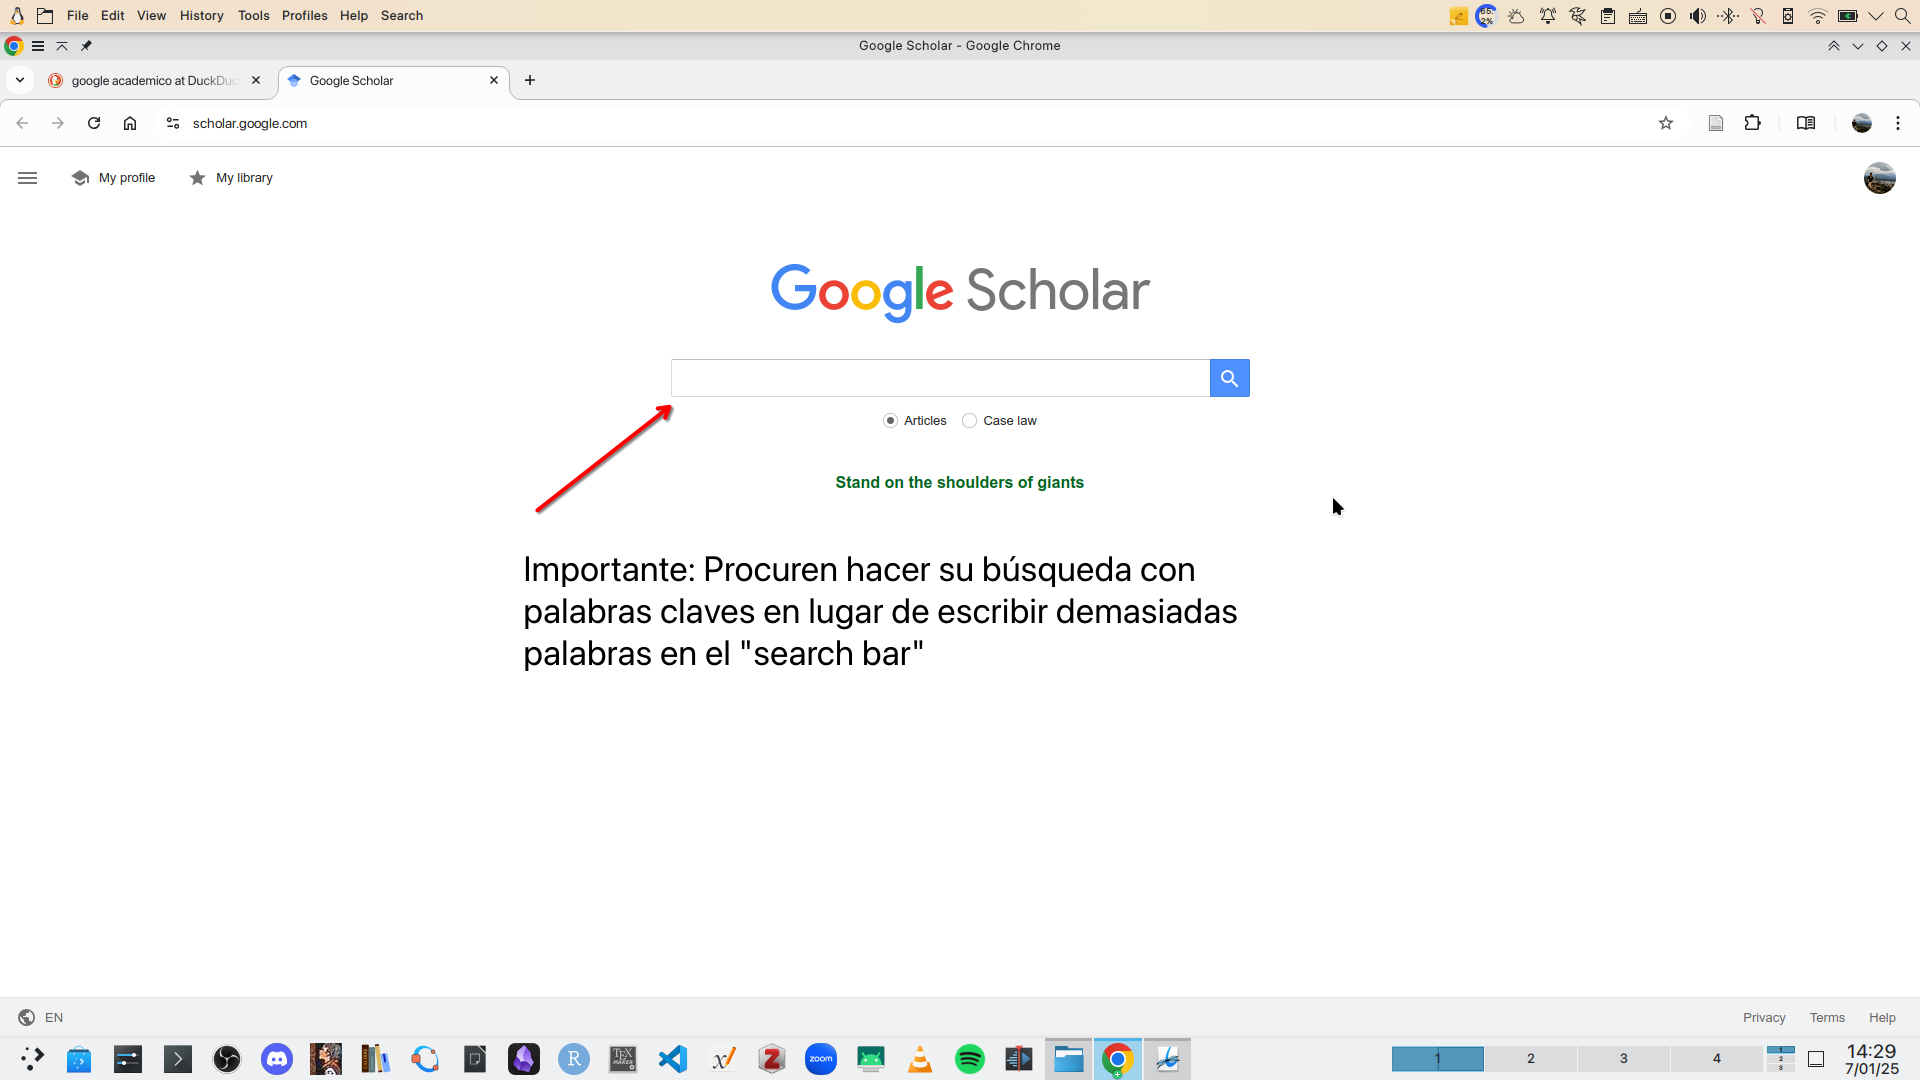
\includegraphics[width=12cm]{screenshot_20250107_142946 1.png}
	\end{figure}
\end{frame}

\begin{frame}{Google Académico}
	\begin{figure}[h!]
		\centering
		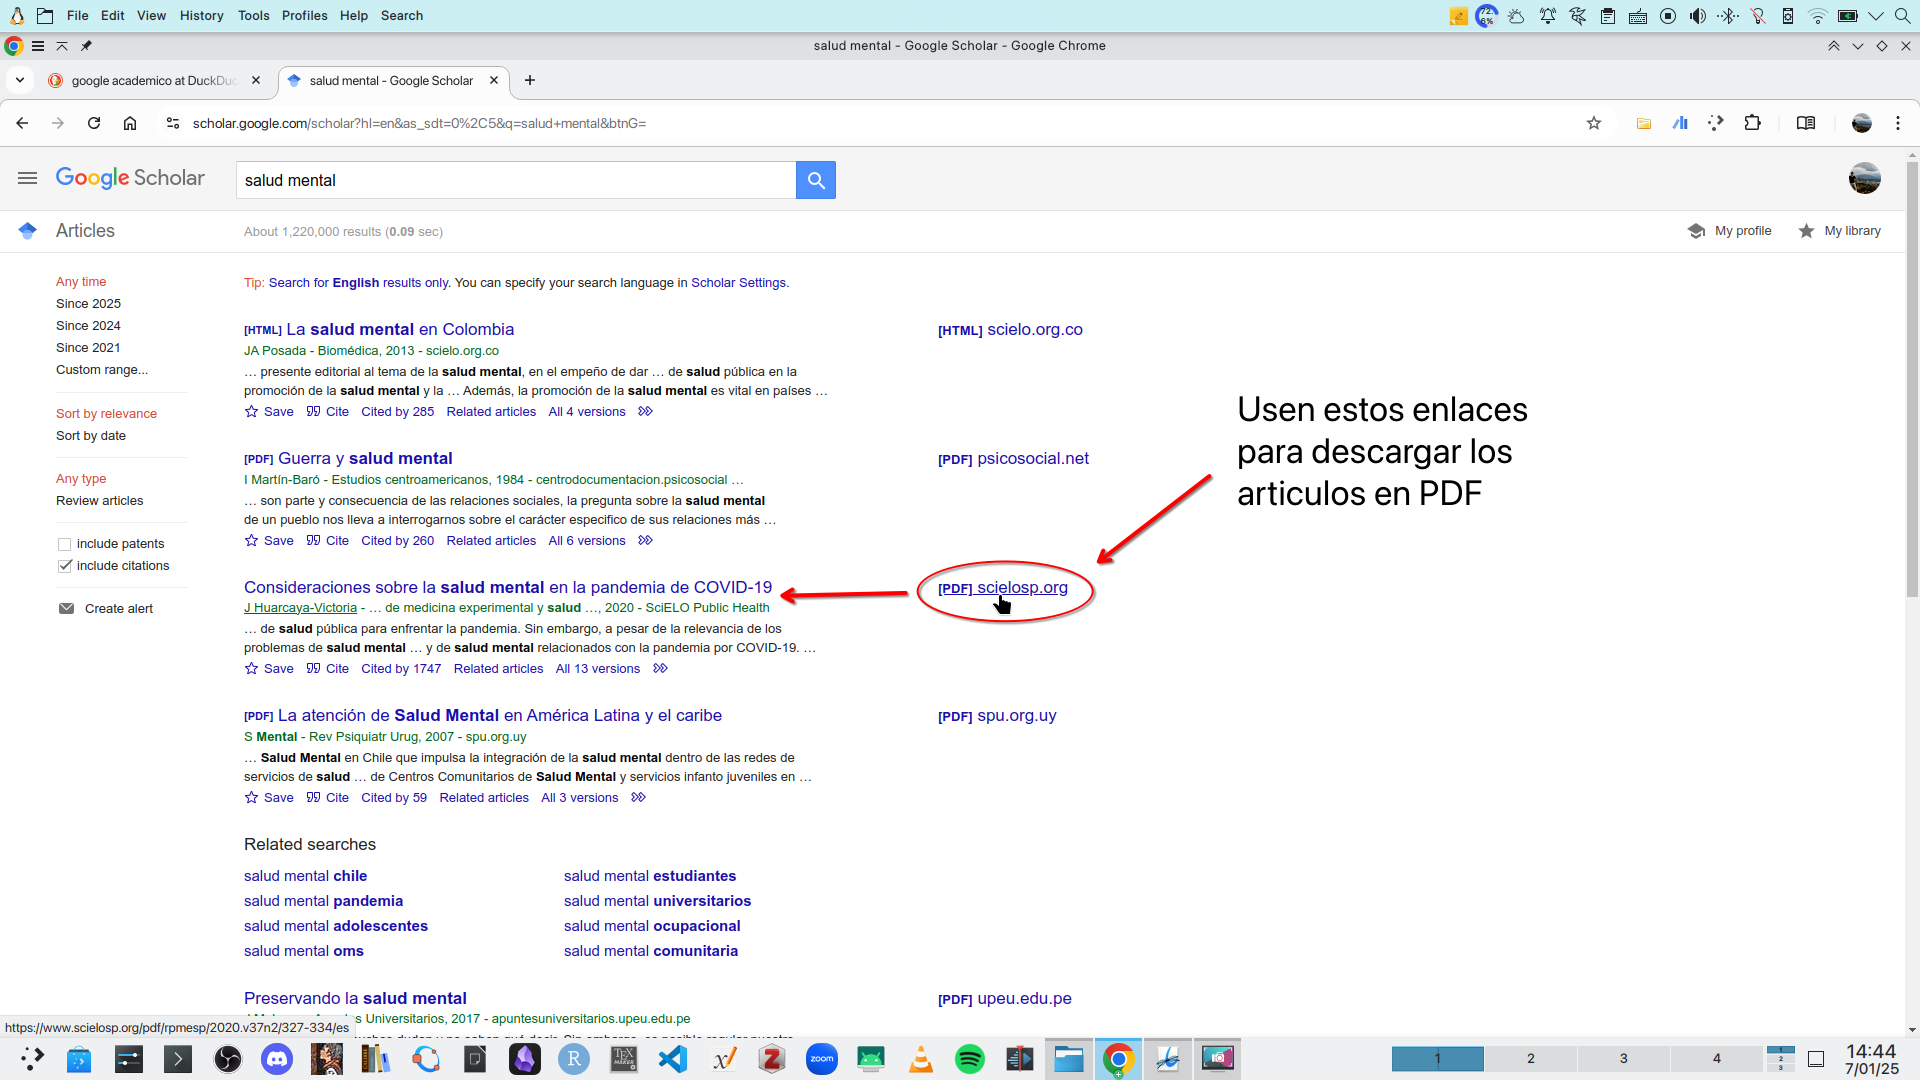
\includegraphics[width=12cm]{screenshot_20250107_144411 1.png}
	\end{figure}
\end{frame}

\begin{frame}{Google Académico}
	\begin{figure}[h!]
		\centering
		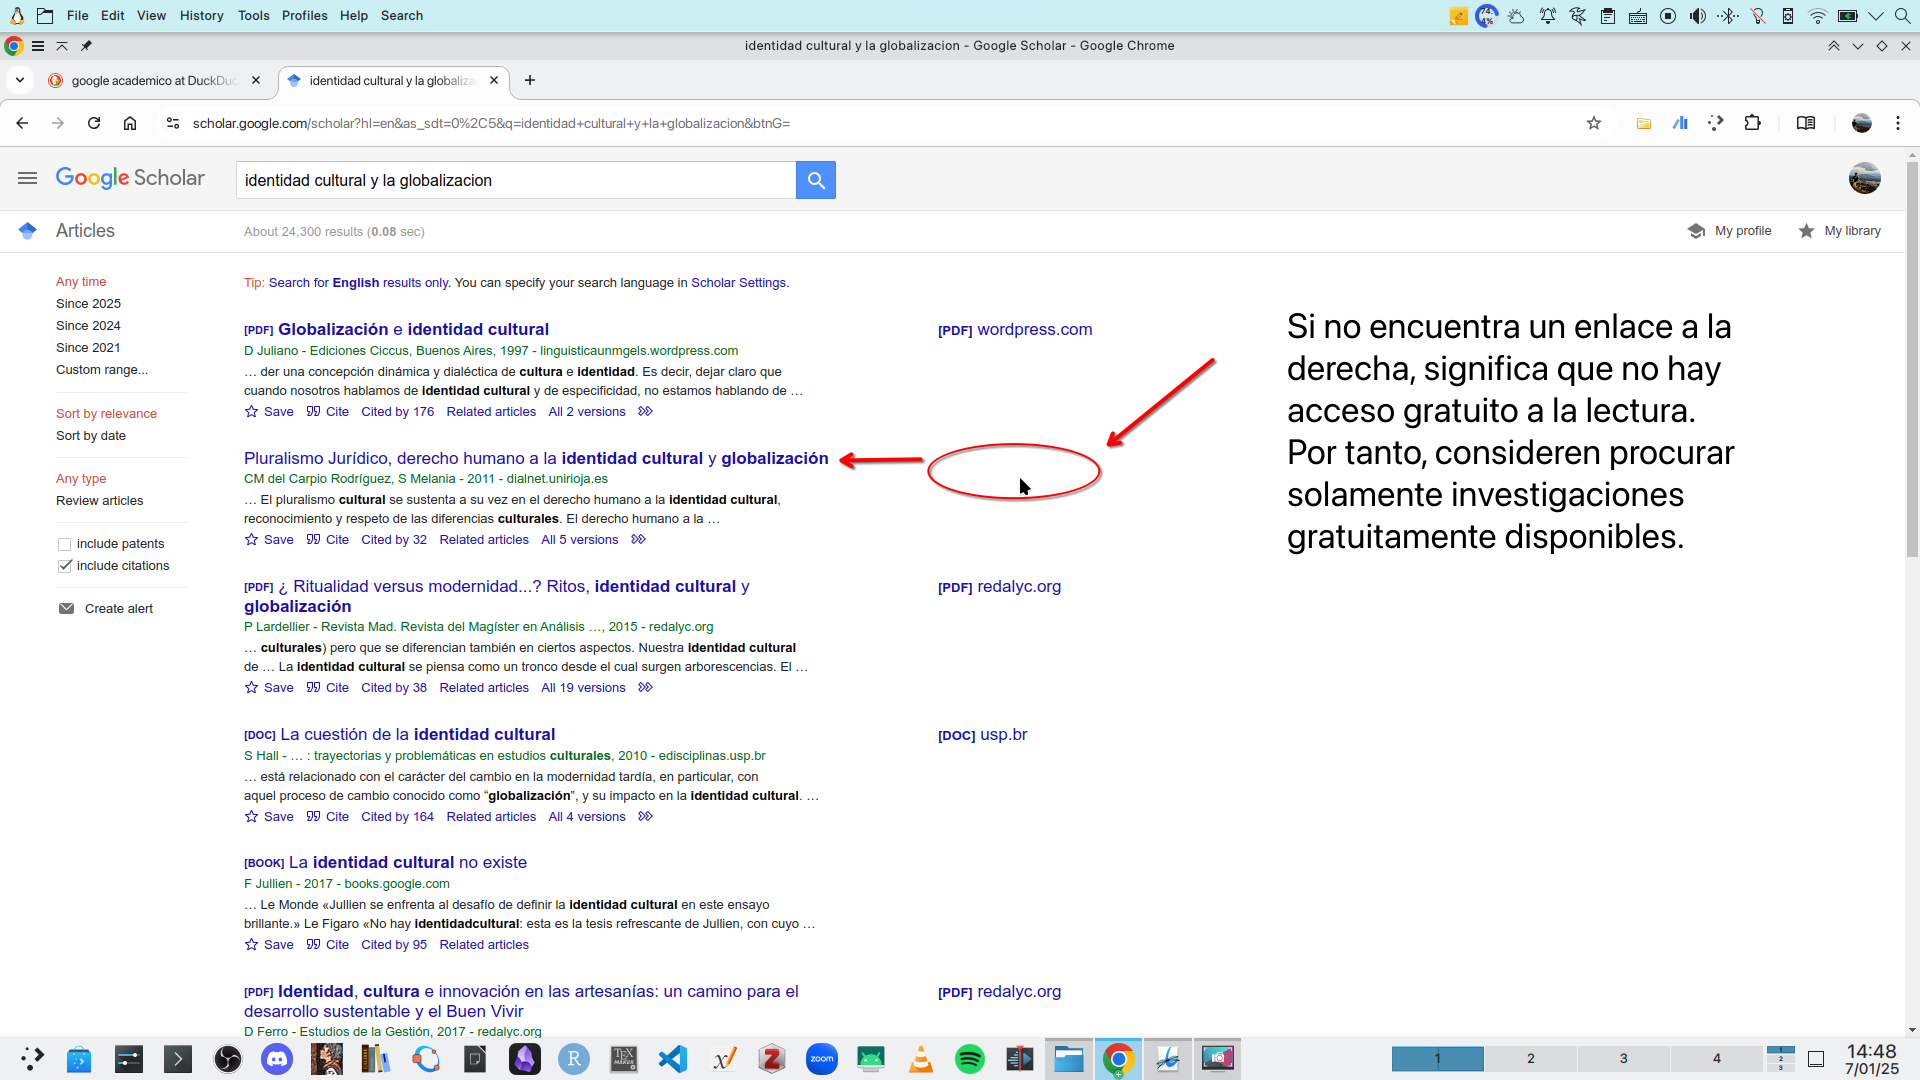
\includegraphics[width=12cm]{screenshot_20250107_144816 4.png}
	\end{figure}
\end{frame}

% Sección 3
\section{Tipos de Trabajos Académicos}

\subsection{Monografía}

% Diapositiva 1: Monografía
\begin{frame}{Monografía}
	\begin{columns}[T]
		\column{0.5\textwidth}
		\centering
		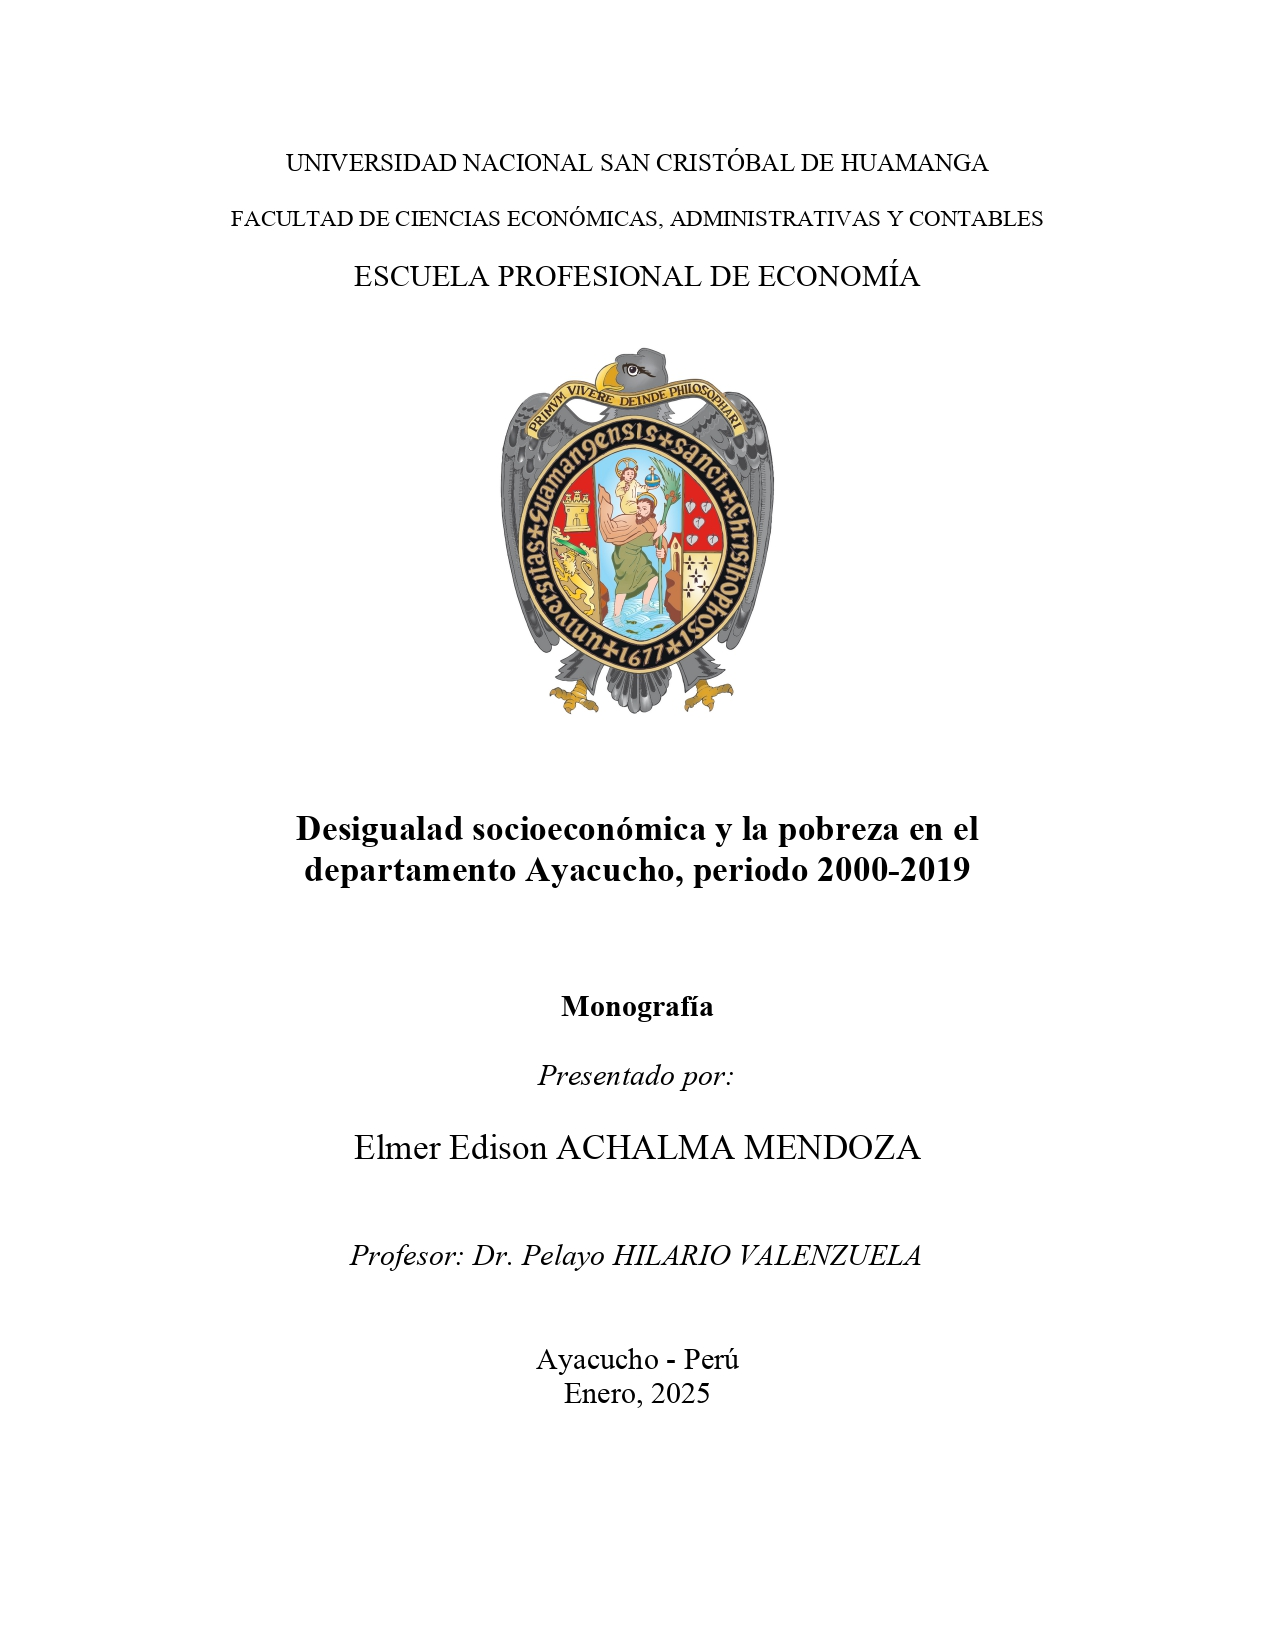
\includegraphics[width=6cm]{caratula monografia.jpg} % Cambia la ruta de la imagen
		\vspace{0.5cm}
		\column{0.5\textwidth}
		\textbf{La monografía} es la iniciación en la investigación sobre un tema específico. Tambien se puede definir como un \textbf{trabajo formal investigativo en el cual debes
			desarrollar un tema}, sostener un punto de vista y llegar a una conclusión.
	\end{columns}
\end{frame}

\begin{frame}{Monografía: Características}
	\textbf{Características principales:}
	\begin{itemize}
		\item Es realizada con claridad y dominio del tema.
		\item Está basada en investigaciones y revisión de literatura relevante.
		\item Posee un estilo académico (APA, MLA, etc.)
		\item Aporta conocimiento original.
		\item Contiene de 8 a 40 páginas.
	\end{itemize}
\end{frame}

\begin{frame}{Monografía: Estructura}

	\textbf{Estructura básica:}
	\begin{itemize}
		\item Portada
		\item Dedicatoria
		\item Índice de contenido (opcional)
		\item Introducción
		\item Cuerpo/Desarrollo
		\item Conclusión
		\item Bibliografía (citada y/o consultada)
		\item Apéndice (opcional)
	\end{itemize}
\end{frame}

\begin{frame}{Monografía: Etapas de escritura en una monografía}

	\begin{columns}[T]
		\column{0.6\textwidth}
		\centering
		\scalebox{0.7}{ % Cambia el 0.8 para reducir o ampliar el tamaño
			\smartdiagram[constellation diagram]{Etapas, 1. Preescritura, 2. Escritura, 3. Contenido, 4. Formato}
		}
		\column{0.4\textwidth}

		Durante el proceso de redactar una monografía, es común revisitar alguna de las
		cuatro etapas. Cada etapa también consiste en varias subetapas. Más adelante
		exploraremos cada paso (y subpaso) del proceso de escribir una monografía.
	\end{columns}

\end{frame}

\begin{frame}{Preescritura}
	\begin{itemize}
		\item Seleccionar un tema
		\item Exponer o argumentar
		\item Investigar
		\item Crear un bosquejo
	\end{itemize}
\end{frame}

\begin{frame}{Preescritura: Selección de tema}

	\begin{block}{Tema}
		El verdadero sentido de elaborar una monografía, es sentir entusiasmo por un tema y trabajar dentro de sus profundos y sinceros intereses. Gracias a un tema predilecto nacen y crecen sus páginas al rededor de el.
	\end{block}

\end{frame}

\begin{frame}{Preescritura: Selección de tema}

	Para escribir una monografía, debes:

	\textbf{1. Seleccionar un tema general}
	\begin{itemize}
		\item Puede que un profesor les indique cuál será el tema compulsorio de la monografía. Para asegurar una buena nota, debe honrar el tema asignado.
		\item En el caso de que el profesor no haya asignado un tema, le corresponde al escritor de la monografía escoger un tema de investigación que le interese y brinde hallazgos válidos a una disciplina académica.
	\end{itemize}

\end{frame}

\begin{frame}{Preescritura: Selección de tema}

	\textbf{2. Investigar literatura relevante}

	Una vez tengas un tema inicial, debes buscar literatura académica sobre dicho
	tema. Todos tus hallazgos te servirán como material cuando estés redactando
	sobre el tema escogido.

	\vspace{0.5cm}

	\textbf{3. Delimitar el tema general a un tema específico}

	Luego de leer suficiente literatura, si el tema inicialmente escogido es
	demasiado general, delimite el tema a uno más específico.

	\vspace{0.5cm}

	\textbf{El tema debe ser de preferencia sencillo, quiere decir específico pero significativo.}

\end{frame}

\begin{frame}{Preescritura: Expositivo o Argumentativo}
	El escritor tiene la libertad de escoger cómo exponer su tema.
	Dependiendo del tema y el contenido recopilado en la revisión de lecturas
	académicas, puede que ciertos temas se presten para ser redactados de manera
	expositiva o argumentativa.

	\vspace{0.5cm}

	\begin{columns}[c]
		\begin{column}{0.45\textwidth}
			\textbf{Expositivo}
			Exponer información de forma clara y
			precisa sobre un tema en particular
			\begin{block}{}
				La historia de la enseñanza del inglés en Perú.
			\end{block}
		\end{column}
		\begin{column}{0.5\textwidth}
			\textbf{Argumentativo}
			Favorecer o criticar una postura dentro de un tema en particular
			\begin{block}{}
				Inglés como lengua extranjera: el método ideal para Perú
			\end{block}
		\end{column}
	\end{columns}
\end{frame}

\begin{frame}{Preescritura: Investigación}
	La investigación es la base del trabajo monográfico. Debe
	realizarse una lectura y un análisis crítico de las fuentes de
	información.

	\vspace{0.5cm}

	Puedes encontrar lecturas académicas confiable en:
	\begin{itemize}
		\item \textbf{Google Académico}: Herramienta de búsqueda académica de Google.
		\item \textbf{Biblioteca Virtual UNSCH}
		\item \textbf{RENATI}: Registro Nacional de Trabajos de Invetigación - 	SUNEDU
		\item \textbf{Scopus}: Base de datos de resúmenes y citas de literatura científica.
		\item \textbf{PubMed}: Repositorio de artículos en ciencias de la salud y biomedicina.
		\item \textbf{ResearchGate}: Red social académica para compartir investigaciones.
	\end{itemize}
\end{frame}

\begin{frame}{Preescritura: Bosquejo}
	Un bosquejo es una guía que ayuda al escritor a determinar cuáles
	son los puntos esenciales que debe discutir en su ensayo y dónde
	debe colocarlos. Por tanto, un buen bosquejo debe pedirle al
	escritor todas las partes de la introducción, los párrafos de
	desarrollo y la conclusión. En la siguiente diapositiva, encontrarán
	un ejemplo de un bosquejo. Más adelante encontrarán una
	diapositiva dedicada a las partes de la introducción, los párrafos de
	desarrollo y la conclusión.
\end{frame}

% Introducción al bosquejo
\begin{frame}{Un bosquejo bien estructurado}
	\begin{itemize}
		\item Sirve como un mapa para desarrollar un escrito claro y coherente.
		\item A continuación, se presenta un ejemplo básico para estructurar:
		      \begin{enumerate}
			      \item Introducción
			      \item Desarrollo
			      \item Conclusión
		      \end{enumerate}
	\end{itemize}
\end{frame}

% Introducción
\begin{frame}{Bosquejo: Introducción}
	\textbf{Oración gancho:} Una frase impactante que capte la atención del lector.
	\begin{block}{}
		El cambio climático se ha convertido en una de las amenazas más graves para la humanidad en el siglo XXI.
	\end{block}

	\textbf{Información necesaria:} Breve contexto que ayude al lector a entender el tema.
	\begin{block}{}
		Las emisiones de gases de efecto invernadero han aumentado drásticamente desde la Revolución Industrial, provocando cambios irreversibles en los ecosistemas.
	\end{block}

	\textbf{Oración tesis:} La idea principal que se desarrollará en el texto.
	\begin{block}{}
		Este ensayo analizará los efectos del cambio climático en la biodiversidad y explorará soluciones para mitigar su impacto.
	\end{block}

\end{frame}

% Desarrollo
\begin{frame}{Bosquejo: Desarrollo}
	Cada párrafo del desarrollo debe incluir:

	\begin{enumerate}
		\item \textbf{Oración temática / Argumento:} Introduce la idea principal que será desarrollada en el párrafo.
		      \begin{block}{}
			      "La deforestación es una de las principales causas del cambio climático y la pérdida de biodiversidad."
		      \end{block}

		\item \textbf{Información que apoye la oración temática:} Evidencias, datos, ejemplos o citas que refuercen el argumento.
		      \begin{block}{}
			      "Según un informe de la FAO (2022), se pierden aproximadamente 10 millones de hectáreas de bosque al año, lo que agrava el calentamiento global y destruye hábitats de especies esenciales."
		      \end{block}
	\end{enumerate}
\end{frame}

% Conclusión
\begin{frame}{Bosquejo: Conclusión}

	\textbf{Oración gancho:} Una frase que recupere la atención del lector al final de la monografía.
	\begin{block}{}
		El futuro del planeta depende de las acciones que tomemos hoy para combatir el cambio climático.
	\end{block}

	\textbf{Información necesaria para el lector:} Resumen breve de los puntos principales discutidos en el texto.
	\begin{block}{}
		La deforestación y las emisiones de gases de efecto invernadero han demostrado ser factores clave en la pérdida de biodiversidad, pero también existen soluciones viables para revertir este daño.
	\end{block}

	\textbf{Oración tesis:} Reformulación de la tesis inicial con un cierre reflexivo.
	\begin{block}{}
		La lucha contra el cambio climático requiere un esfuerzo conjunto entre gobiernos, empresas y ciudadanos para garantizar un futuro sostenible.
	\end{block}
\end{frame}

\begin{frame}{Escritura: Introducción}

	\begin{columns}[c]
		\begin{column}{0.45\textwidth}
			\textbf{Oración gancho}
			\begin{itemize}
				\item Motiva al lector a leer la monografía
				\item Presenta un dato llamativo del tema a discutirse
			\end{itemize}
			\textbf{Oración tesis}
			\begin{itemize}
				\item Presenta la idea/motivación principal de la monografía
			\end{itemize}
		\end{column}
		\begin{column}{0.5\textwidth}
			\textbf{Información necesaria para el lector:}
			\begin{itemize}
				\item Autores relevantes
				\item Título de obra(s) discutida(s)
				\item Perspectivas académicas
				\item Definiciones de vocabulario necesario. Etc
			\end{itemize}
		\end{column}
	\end{columns}
\end{frame}

\begin{frame}{Escritura: Desarrollo}
	\textbf{Párrafo(s)}
	\begin{itemize}
		\item 	\textbf{Oración temática / Argumento}
		      \begin{itemize}
			      \item Apoya la idea principal presentada en la introducción
			      \item Es el único tema que se desarrollará en el párrafo donde se encuentre.(Cada tema que te ayude a demostrar tu idea principal debe desarrollarse en su propio párrafo. Esto se hace para mantener organización y claridad.)
		      \end{itemize}
		\item \textbf{Información que apoye a la oración temática}

		      \begin{itemize}
			      \item Las citas pueden ser directas o parafraseadas. Más adelante se expondrá la diferencia entre ambos estilos de citar.
			      \item Cada cita debe ser seguida por una interpretación de la cita. \textbf{No debes citar sin propósito.} Se cita para evidenciar y apoyar el punto que se presenta en la oración temática.
		      \end{itemize}
	\end{itemize}

\end{frame}

\begin{frame}{Escritura: Conclusión}
	Una conclusión debe tener los siguientes elementos:
	\begin{itemize}
		\item  \textbf{Resumen de información importante}
		      \begin{itemize}
			      \item Datos esenciales que el lector debe preservar de tu monografía. Ojo, no debes repetir todos los puntos discutidos en los párrafos del desarrollo.
		      \end{itemize}
		\item \textbf{Reiteración de la tesis}
		      \begin{itemize}
			      \item Reiteramos la tesis con el fin de demostrar que se cumplió el motivo principal
			            de la monografía. Una manera eficiente de cumplir con el resumen de la
			            información importante y la reiteración de la tesis es estableciendo una
			            relación entre ellas. El motivo de tu monografía se demostró a través de los
			            puntos que desarrollaste en el escrito.
		      \end{itemize}
		\item \textbf{Oración de cierre}
		      \begin{itemize}
			      \item Dependiendo del tema que estés discutiendo en la monografía, puedes:
			      \item Discutir qué podrían hacer en las próximas investigaciones
			      \item Hacer críticas constructivas sobre tu análisis o el análisis de las lecturas corroboradas
			      \item Ofrecer tu opinión respecto al tema
		      \end{itemize}
	\end{itemize}
\end{frame}

\begin{frame}{Edición de contenido}
	Una vez hayas terminado de escribir tu primer borrador, debes:
	\begin{itemize}
		\item \textbf{Cotejar el buen uso de la gramática}
		      \begin{itemize}
			      \item Buscar y corregir ‘typos’, cambiar registros casuales por sus equivalentes formales y asegurar uso correcto de puntuación.
		      \end{itemize}

		\item \textbf{Reorganizar contenido de ser necesario}
		      \begin{itemize}
			      \item Revisa si el contenido del borrador coincide con el bosquejo previamente preparado.
		      \end{itemize}

		\item \textbf{Evitar cometer plagio}
		      \begin{itemize}
			      \item Si una idea no es tuya, hay que indicar de quién es.
		      \end{itemize}

		\item \textbf{Usar un diccionario}
		      \begin{itemize}
			      \item Te permite buscar vocabulario claro y preciso.
			      \item Ayuda a evitar el sobreuso de las palabras.
		      \end{itemize}
	\end{itemize}
\end{frame}

\subsection{Informe Académico y Profesional}

% Diapositiva 2: Informe Académico y Profesional
\begin{frame}{Informe de laboratorio}
	\begin{columns}[c]
		\begin{column}{0.45\textwidth}
			\centering
			
\includegraphics[width=6cm]{caratula informe.jpg} % Cambia la ruta de la imagen
			\vspace{0.5cm}
		\end{column}
		\begin{column}{0.5\textwidth}
			\textbf{INFORME:} Un informe de laboratorio, también llamado informe científico, \textbf{es un documento estructurado destinado a comunicar de forma eficiente los hallazgos de una investigación}. El mismo sigue un formato en especifico con la finalidad de llegar a la comunidad científica de manera uniforme.
		\end{column}
	\end{columns}
\end{frame}

\begin{frame}{Propósitos de un informe}
	\textbf{Propósitos de un informe:}
	\begin{itemize}
		\item Describe los criterios, características y metodología de una investigación.
		\item Actúa como instrumento para comunicar los resultados de la misma.
		\item Constituyen fuentes de información confiables para futuras investigaciones.
	\end{itemize}
\end{frame}

\begin{frame}{Características del informe}
	\textbf{Características principales:}
	\begin{itemize}
		\item Escrito con claridad y precisión (\textbf{No vocabulario rebuscado})
		\item Objetivo concreto (\textbf{Debe ir acorde con el experimento})
		\item Citar el autor o autores (\textbf{Hacer referencias a ellos al final del trabajo en la parte de literatura citada})
	\end{itemize}
\end{frame}

\begin{frame}{Partes de un informe}
	\textbf{Estructura típica:}
	\begin{itemize}
		\item Portada. (1)
		\item Resumen. (1)
		\item Tabla de contendido (Opcional)
		\item Introducción. (1)
		\item Materiales y Métodos (2)
		\item Resultados (Máximo 4)
		\item Discusión (1)
		\item Referencia (1)
		\item Anexos (si aplica).
	\end{itemize}
	Total máximo de páginas (10)
\end{frame}

\begin{frame}{Portada}
	\begin{itemize}
		\item Nombre de la Universidad
		\item Nombre de la facultad
		\item Nombre de la escuela profesional
		\item logo
		\item Título
		\item Nombre del docente
		\item Nombre del estudiante
		\item Código de curso
		\item Fecha de ejecución y entrega
		\item Lugar y fecha
	\end{itemize}
\end{frame}

\begin{frame}{Resumen}
	\begin{itemize}
		\item Primera parte del contenido
		\item Es lo último que se escribe
		\item Debe incluir:
		      \begin{itemize}
			      \item Breve introducción
			      \item Objetivos del trabajo
			      \item Metodología empleada
			      \item Resultados logrados
			      \item Conclusiones
		      \end{itemize}
	\end{itemize}
	250 palabras o menos.
\end{frame}

\begin{frame}{Tabla de Contenido}
	\begin{itemize}
		\item Refiere al lector las partes del informe, presentando la forma en que está organizado
		\item Debe especificar exactamente en que página comienza la información que busca el lector
		\item Una sola página.
		\item Identifica en parte superior “Tabla de Contenido”
	\end{itemize}
\end{frame}

\begin{frame}{Introducción del Informe}
	\begin{itemize}
		\item Se debe redactar en una nueva página del informe.
		\item El texto debe escribirse en tiempo presente.
		\item Proporciona una visión general del contenido del informe.
		\item Establece el propósito y los objetivos del documento.
		\item Debe ser clara, concisa y relevante.
	\end{itemize}
\end{frame}


\begin{frame}{Materiales y Métodos}
	\begin{itemize}
		\item \textbf{Descripción del diseño experimental:}
		      Breve introducción que explique la estructura y enfoque del diseño utilizado.

		\item \textbf{Flujograma:}
		      \begin{itemize}
			      \item Debe ser general y claro.
			      \item Presentar los pasos de forma breve y precisa.
			      \item No incluir cantidades ni detalles excesivos.
			      \item Limitar a 4-6 pasos clave.
		      \end{itemize}
		\item \textbf{Párrafo descriptivo:}
		      \begin{itemize}
			      \item Proveer una explicación específica de los procedimientos.
			      \item Redactar de manera técnica y concisa.
		      \end{itemize}
	\end{itemize}
\end{frame}

\begin{frame}{Resultados}
	\begin{itemize}
		\item \textbf{Descripción breve del experimento:} Redactada en pasado, proporcionando el contexto esencial del procedimiento realizado.

		\item \textbf{Resumen de los datos recopilados:} Explicación concisa sobre cómo se obtuvieron los datos clave durante el experimento.

		\item \textbf{Estadísticas aplicadas:} Detalle de los métodos estadísticos utilizados para analizar los datos, resaltando su relevancia.
	\end{itemize}
	\begin{columns}[c]
		\begin{column}{0.45\textwidth}
			\textbf{Figuras:} Representación visual con un análisis rápido de tendencias y el significado de los datos. Fotografías de los procedimientos en el laboratorio.

			\textbf{Tablas:} Contienen cifras comparativas y datos que no presentan tendencias.
		\end{column}
		\begin{column}{0.5\textwidth}
			\centering
			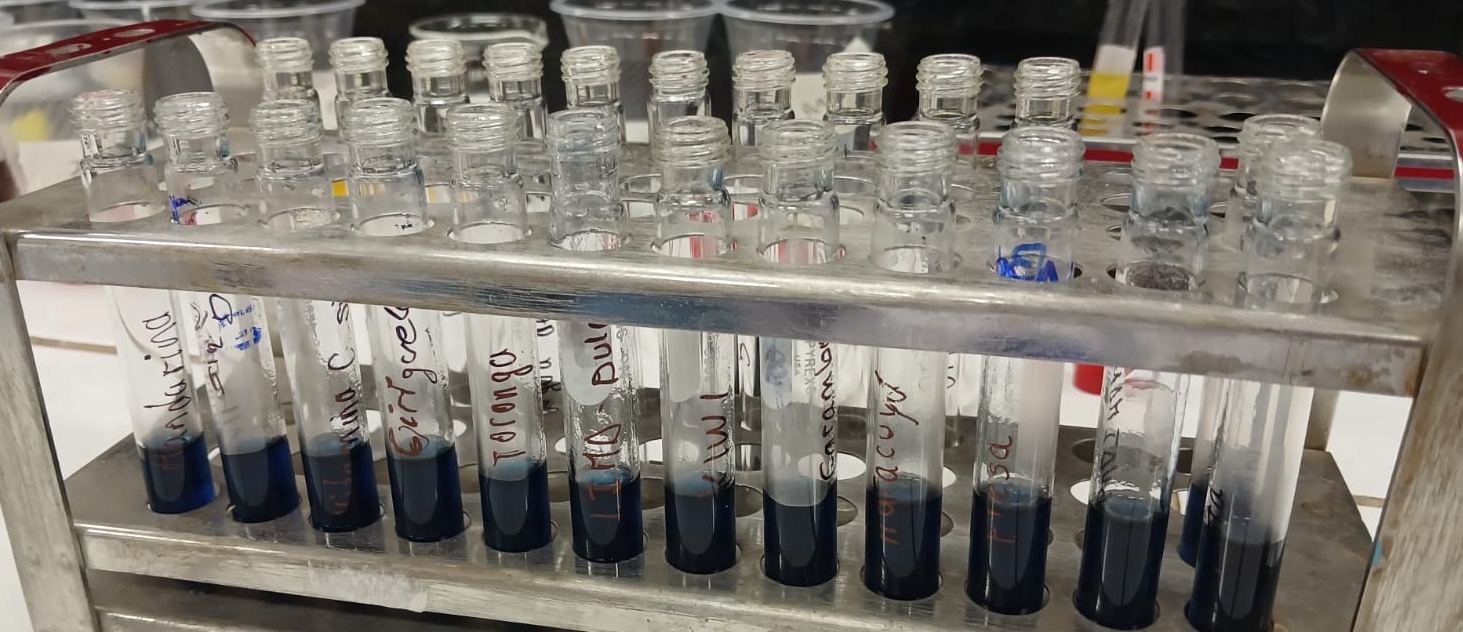
\includegraphics[width=6cm]{resultado01.png} % Cambia la ruta de la imagen.
		\end{column}
	\end{columns}
\end{frame}

\begin{frame}{Discusión}
	\begin{itemize}
		\item Presentar principios
		\item Analizar resultados (NO repetirlos)
		\item Señalar excepciones o falta de correlación.
		\item Comparar datos con:
		      \begin{itemize}
			      \item Otros estudiantes
			      \item Literatura científica
		      \end{itemize}
		\item El último párrafo debe expresar de forma breve las conclusiones
		      \begin{itemize}
			      \item Resumir evidencia de estas
			      \item Buscar principios que las expliquen
		      \end{itemize}
		\item Debe responder a los objetivos del ejercicio.
	\end{itemize}
\end{frame}

\begin{frame}{Literatura Citada}
	\begin{itemize}
		\item \textbf{Propósito}
		      \begin{itemize}
			      \item Respaldar tus expresiones y evidencia que has investigado
			      \item Permite al lector buscar mayor información o aclarar dudas
		      \end{itemize}
		      \textbf{Solo citar fuente que hayas leído y usado en el trabajo}

		      Las fuentes citadas tienen que estar en el informe: Introducción, materiales y
		      métodos y discusión
	\end{itemize}
\end{frame}

\subsection{Tesis}

% Diapositiva 3: Tesis
\subsection{Diferencias y Similitudes}

% Diapositiva 4: Diferencias y Similitudes
\begin{frame}{Diferencias y Similitudes entre los Tipos de Documentos}
	\textbf{Diferencias:}
	\begin{itemize}
		\item \textbf{Monografía:} Enfoque en revisión bibliográfica y análisis crítico.
		\item \textbf{Tesis:} Basada en investigación original, con rigor metodológico.
		\item \textbf{Informe:} Orientado a describir y comunicar resultados de una actividad específica.
	\end{itemize}
	\textbf{Similitudes:}
	\begin{itemize}
		\item Todos requieren claridad, coherencia y estructura definida.
		\item Exigen el uso adecuado de referencias y citas.
		\item Contribuyen al desarrollo académico o profesional del autor.
	\end{itemize}
\end{frame}

% Sección 4
\section{Normas APA Séptima Edición}
\begin{frame}{¿Qué es el APA?}
	\centering
	
\includegraphics[width=4cm]{logoapa.png}
	\vspace{0.5cm}
	\textbf{Asociación Americana de Psicología}
	\begin{itemize}
		\item Es una \textbf{organización científica y profesional de psicólogos} estadounidenses.
		\item La APA fue \textbf{fundada en julio de 1892} en una Universidad de Clark.
		\item La \textbf{mayor asociación mundial de psicólogos del mundo.}
		\item La función de la APA es el avance de la psicología como ciencia y profesión, y también la promoción de la salud, la educación y el bienestar humano.
	\end{itemize}
\end{frame}

\begin{frame}{Historia}
	\textbf{El estilo APA se originó en 1929}, al realizar la publicación de las primeras pautas en \textbf{un artículo de siete páginas en el Boletín Psicológico.}
	\centering
	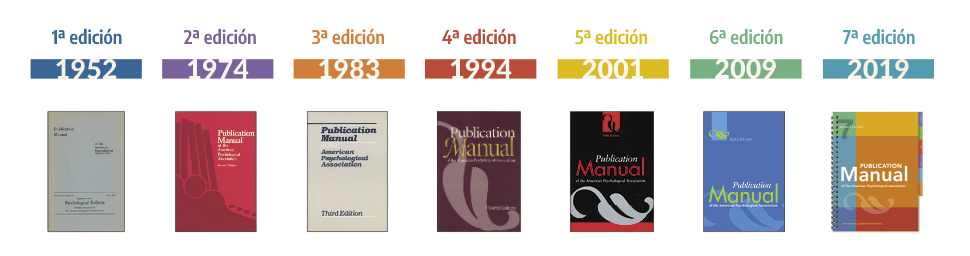
\includegraphics[width=12cm]{normas apa todas ediciones.png} % Imagen que contiene las ediciones
	% Fechas dinámicas
	\vspace{0.5cm} % Ajusta el espacio vertical
	\only<2>{\textbf{1952 - Primera edición}}
	\only<3>{\textbf{1974 - Segunda edición (22 años después)}}
	\only<4>{\textbf{1983 - Tercera edición (9 años después)}}
	\only<5>{\textbf{1994 - Cuarta edición (11 años después)} \\ Versión en español (1998):  Primera edición}
	\only<6>{\textbf{2001 - Quinta edición (7 años después)}}
	\only<7>{\textbf{2009 - Sexta edición (8 años después)} \\ Versión en español (2010):  Tercera edición, por Manual Moderno}
	\only<8>{\textbf{2019 - Sexta edición (10 años después) \\ VIGENTE}}
\end{frame}

\begin{frame}{¿Por qué son necesarias las normas APA?}

	Las Normas APA nos brindan un procedimiento o normas de estilo con el objetivo
	de estandarizar los documentos para facilitar la comprensión de la lectura.
	\begin{itemize}
		\item La uniformidad y la coherencia permite a los lectores centrarse en las ideas.
		\item Las pautas de estilo apoyan a los autores a acreditar completamente la información.
		\item Las ideas fluyen lógicamente, las fuentes se acrediten adecuadamente y los documentos se organizan de manera predecible y consistente.
	\end{itemize}
\end{frame}

\begin{frame}{¿Por qué son necesarias las normas APA?}
	Las Normas APA nos brindan un procedimiento o normas de estilo \textbf{con el objetivo de estandarizar los documentos para facilitar la comprensión de la lectura.}
	\begin{columns} % Inicia las columnas
		\column{0.3\textwidth} % Primera columna ocupa el 40% del ancho
		\centering
		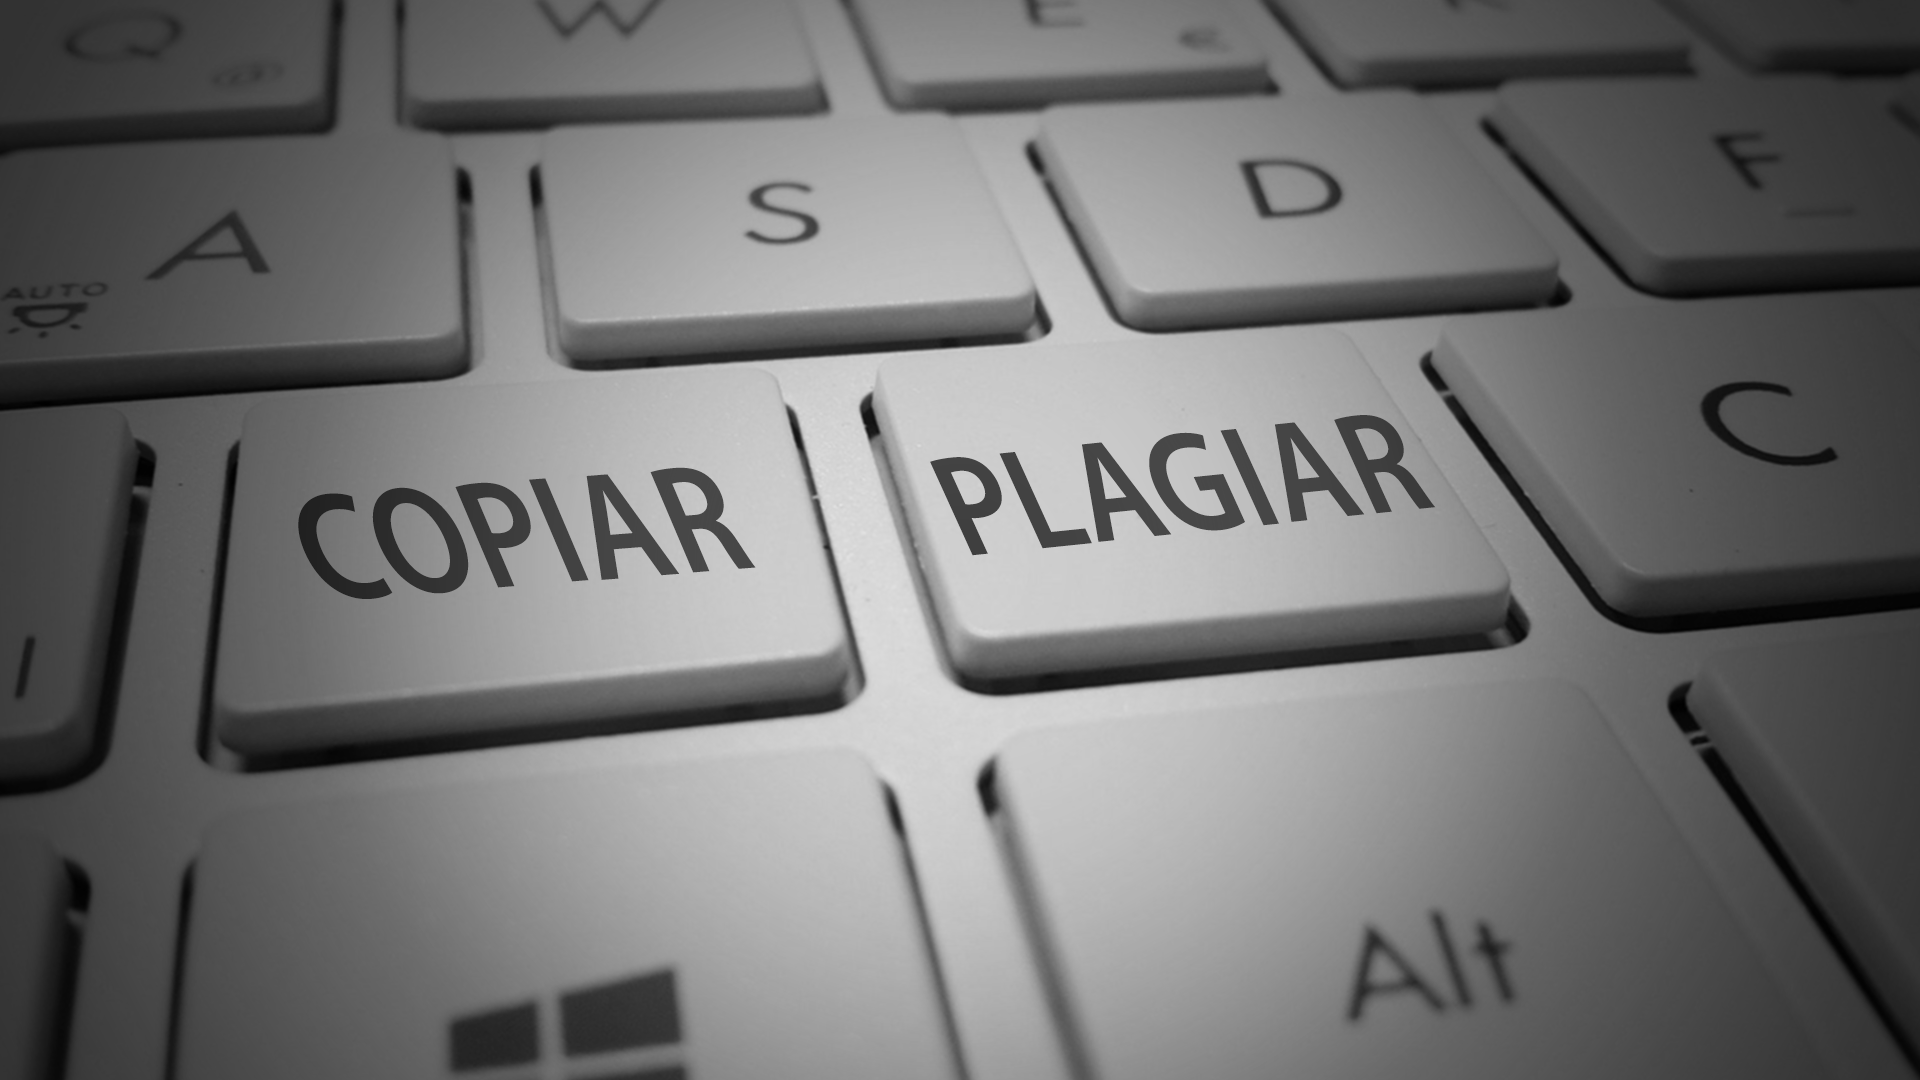
\includegraphics[width=\textwidth]{figura01.png} % Inserta la imagen (ajusta el nombre del archivo y el tamaño)
		\column{0.7\textwidth} % Segunda columna ocupa el 60% del ancho
		\begin{itemize}
			\item La uniformidad y la coherencia permite a los lectores centrarse en las ideas.
			\item Las pautas de estilo apoyan a los autores a acreditar completamente la información.
			\item Las ideas fluyen lógicamente, las fuentes se acrediten adecuadamente y los documentos se organizan de manera predecible y consistente.
			\item Contribuyendo en el uso ético y legas de la información.
		\end{itemize}
	\end{columns}
\end{frame}

% Sección 5
\section{Estructura}
\begin{frame}{Estructura de un documento}
	\centering
	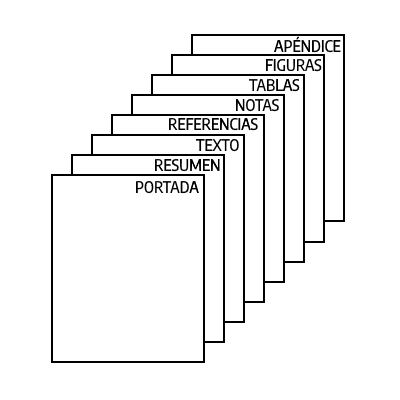
\includegraphics[width=6cm]{figura01 normas apa estructura.png}
	{\color{blue} Recuerda que estos elementos pueden modificarse de acuerdo con las exigencias de los docentes, instituciones o revistas.}
\end{frame}

% Sección 6
\section{Formato}
\begin{frame}{Formato}

\end{frame}

%----------------------------------------------------------------------------------------
\end{document}